\chapter{Evaluation}\label{ch:eval}

%This chapter is mainly provided for the purpose of showing a typical thesis
%structure. There are no more thesis requirements described.

\section {Considered Evaluation Methods}

We considered two different ways of evaluating our system.

The first method was to simulate real users by creating Facebook accounts and attempting to mimic behaviour of each user type. We would then create a ground truth regarding how that type of user would like their feed ranked and compare the output of our ranking algorithm to the ground truth. We found quite a few flaws in this method, the major one being how difficult it would be to simulate a real user. Creating social interactions and simulating connections between users would prove very difficult. On top of this, the ground truths that we would be creating could be affected by confirmation bias. This left us with a very questionable evaluation method, so we arrived at our second one.

The second evaluation method takes the form of gathering real users and performing a form of usability test. In this test, we will ask participants to order their feeds how they would like it to be seen, this forms an unbiased ground truth. We then run our ranking algorithm on their feeds and compare the ground truth they gave us earlier to the output. In addition to this ground truth comparison, we will ask the user to compare our ranking algorithm with the one provided by Facebook, without telling them which is which. This will give us some subjective results as to whether our ranking algorithm has succeeded in personalising the user's feed.

\section{Evaluation Approach}

From the two methods that were considered, we chose to use our second method. However, we decided to use a modified version of it since the purpose of our algorithm is to provide different views of the user’s feed, not necessarily a better algorithm than Facebook’s which would prove extremely difficult considering the amount of data, time and resources put into their algorithm. 

We gathered users and conducted a usability test on each of them. We pulled 50 items from their feed and had each user choose 10 items that they would like to see at the top of the feed. We then used our ranking algorithm and measured how many of the items they chose ended up in the top 10, 25 and finally 30 of our ranked feed. If we have a majority of the items that interest them at the top of the feed then we can say that our algorithm was a success.

We performed our evaluation on a very small scale as we felt that the background research connected to our design decisions are sufficient to back up our algorithm and our intention was for these sessions to act as a simple sanity check for our application rather than a large scale verification of our algorithm.

\begin{center}
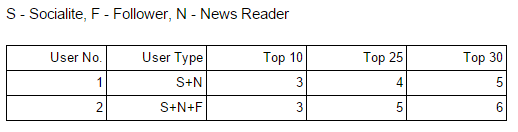
\includegraphics[scale=0.8]{images/results.png}
\captionof{figure}{Table of sample users}
\end{center}

In figure 5.1 the top 10 refers to the the amount of items that the user has chosen that appeared in the top 10. The top 25 refers to the amount of items that the user has chosen that appeared in the top 25. Similarly top 30 refers to the amount of items that the user has chosen that appeared in the top 30 items of the feed in our ranking algorithm. From the table we can see that our algorithm is not performing as well as intended. Approximately 30 percent of the items in the feed that the user enjoys is at the top 3 with 50 percent  being in the top 25. 

\section{Discussion}

From our results, it may appear as though our algorithm is not performing well, however, on further analysis, when we look at the posts the user had interest in and the selected type, we find that users don’t seem to be selecting the user type that best describes themselves. Some users chose the user type to be socialite, yet they have selected many posts that belong to the user type of Follower. Since we also pull a small amount of feed items compared to the large pool that Facebook has, there will likely be many items that the user does not want to see. This makes it difficult for them to select the best 10 items as they may not like any of the 50 that we have provided. This idea could skew our results.
